\documentclass[10pt]{article}
\usepackage[T1]{fontenc}
\usepackage[francais]{babel}
\usepackage{array}
\usepackage{shortvrb}
\usepackage{listings}
\usepackage[fleqn]{amsmath}
\usepackage{amsfonts}
\usepackage{fullpage}
\usepackage{enumerate}
\usepackage{graphicx}             % import, scale, and rotate graphics
\usepackage{subfigure}            % group figures
\usepackage{alltt}
\usepackage{url}
\usepackage{indentfirst}
\usepackage{eurosym}
\usepackage{amsmath} 
\usepackage{float}
\usepackage{caption}

%Définition du c pour les "listings"
\usepackage{listings}
\usepackage{xcolor}
\definecolor{mGreen}{rgb}{0,0.6,0}
\definecolor{mGray}{rgb}{0.5,0.5,0.5}
\definecolor{mPurple}{rgb}{0.58,0,0.82}
\definecolor{backgroundColour}{rgb}{0.95,0.95,0.92}

\lstdefinestyle{CStyle}{
    backgroundcolor=\color{backgroundColour},   
    commentstyle=\color{mGreen},
    keywordstyle=\color{magenta},
    numberstyle=\tiny\color{mGray},
    stringstyle=\color{mPurple},
    basicstyle=\footnotesize,
    breakatwhitespace=false,         
    breaklines=true,                 
    captionpos=b,                    
    keepspaces=true,                 
    numbers=left,                    
    numbersep=5pt,                  
    showspaces=false,                
    showstringspaces=false,
    showtabs=false,                  
    tabsize=2,
    language=C
}


%\usepackage[french,onelanguage,ruled,vlined]{algorithm2e}
%\usepackage{clrscode3e}
%\usepackage{algorithm, algpseudocode}
%\usepackage{tabular}
\usepackage[utf8]{inputenc}
\usepackage{clrscode3e}
%\usepackage{algpseudocode}

% changement de la numerotation
\setcounter{secnumdepth}{5}
%\renewcommand{\thechapter}{\Alph{chapter}}
%\renewcommand{\thesection}{\Roman{section})}
%\renewcommand{\thesubsection}{\arabic{subsection})}


%\title{\textbf{INFO2050 : Rapport numéro un programmation avancée}}
%\author{Antoine Sadzot}
%\date{30-10-17}
\begin{document}
\begin{titlepage}

   \begin{figure}[htbp]
      \centering
      
\includegraphics{uliege-logo-couleurs-300.jpg}
   \end{figure}
  	
  	\hfill

	\begin{center}
		\vfill
		\textbf{
		\Huge{INFO2050-1 - Programmation Avancée}}\\
		\bigskip
		\huge{Projet 2: Structures de Données}\\
		\bigskip %saut de ligne
		\smallskip
		\Large{Aliaksei Mazurchyk\\Antoine Sadzot}\\
		\bigskip
		\smallskip
		\large{\today}\\%date
		\vfill
		\large{Université de Liège}
	\end{center}
\end{titlepage}
\clearpage
\clearpage

\section{Analyse Théorique}
\subsection{Variante d'union-find à base d'arbres choisie}
	La version de l'union-find en arbre implémentée est une version améliorée. Comme dans la version de base chaque élément pointe vers son parent. Lors d'une union de sous-ensembles, les racines des deux arbres sont fusionnés, un parent se retrouve donc avec deux enfants.
	
	\paragraph{Rang}			
	La première amélioration consiste à associer un rang a chaque élément. Cela permet d'optimiser la fusion. L'union-find de base pouvait être fort déséquilibré, ce qui rendais l'appel Find() assez long. L'ajout d'un rang permet d'équilibrer l'arbre lors de l'union. 
	
	Au début tous les éléments ont un rang 0. Lors d'une fusion de deux arbres de même hauteur, le rang de la nouvelle racine est incrémenté de 1. Si les rangs sont différents, l'arbre ayant le rang le plus petit est ajouté à la racine de l'arbre le plus grand. Cela permet d'équilibrer la structure au fur et à mesure de la construction et ainsi de diminuer la hauteur maximale.
	
	\paragraph{Compression de chemin}
	Cette seconde amélioration consiste à utiliser la fonction Find() pour aplatir l'arbre. Cela ce fait lors de l'appel récursif, la racine de l'arbre remonte dans la call-stack et est définie en tant que parent de chaque neud parcouru. De cette manière, tous les éléments parcouru par un Find(), pointeront directement vers la racine et nécessiteront donc un temps constant pour récupérer cette dernière.

\subsection{Complexités en temps de ufUnion et ufFind}

\subsubsection{Implémentation à base de listes chainées}

\begin{description}
\item[ufFind :] Dans tous les cas, la complexité est $\Theta(1)$
\item[ufUnion :] Dans le meilleur cas, le plus petit ensemble à lier à la suite du second ensemble ne contient qu'un élément. La complexité dans le meilleur cas est donc $\Theta(1)$. Dans le pire cas, l'ensemble à lier à la suite du second ensemble est de taille N/2, N étant le nombre d'éléments du labyrinthe. La complexité dans le pire cas est donc $\Theta(N/2)$.
\end{description}
\subsubsection{Implémentation à base d'arbres}
\begin{description}
\item[ufFind :] Dans le meilleur des cas, la complexité est $\Theta(1)$. Dans le pire est est $\mathcal{O}(h)$, avec $h$ comme auteur de l'arbre. 
\item[ufUnion :] Dans le meilleur des cas, la complexité est $\Theta(1)$. Dans le pire est est $\mathcal{O}(n + log(n))$.
\item[Complexité combinée:] Dans le meilleur des cas, la complexité est $\Theta(1)$. Dans le pire elle est $\Omega( \alpha(n))$, ce qui équivaut à un temps constant car $\alpha(n)$ (fonction d'Ackermann inversée) a une croissance extrêmement lente. En pratique: $\alpha(2^{65536}) = 5$ ce qui garanti une complexité $\Theta(5)$. Cette complexité vaut pour l'\emph{Union} et le \emph{Find}, car les deux améliorations sont complémentaire et l'un tire parti des améliorations de l'autre. Ceci fut démontré par Fredman et Saks en 1989.

\paragraph{Sources} 
\begin{itemize}
\item[•] \url{en.wikipedia.org/wiki/Disjoint-set_data_structure}
\item[•] \url{fr.slideshare.net/NikitaShpilevoy/algorithms-union-find}
\item[•] \url{fr.slideshare.net/WeiLi73/time-complexity-of-union-find-55858534}
\item[•] \url{github.com/emintham/Papers/blob/master/Fredman%2CSaks-%20The%20cell%20probe%20complexity%20of%20dynamic%20data%20structures.pdf}
\end{itemize}

\end{description}
\subsection{Implémentation de la structure du labyrinthe}
Les données du labyrinthe sont stockées dans la structure Maze.
\begin{lstlisting}[style=CStyle]
struct maze_t {
    UnionFind *union_Find;
     struct Walls *myWalls;
     size_t size;
     size_t number_inner_walls;
     size_t number_open_walls;
};
\end{lstlisting}

La structure "maze\_t" contient la structure "UnionFind", qui sera décrite pour chaque implémentation par la suite. Elle contient également la structure "Walls" qui est un vecteur enregistrant tous les murs internes du labyrinthe. La variable "size" contient la taille du labyrinthe. La variable "number\_inner\_walls" contient le nombre de mur internes du labyrinthe. C'est également la taille du vecteur de type "Walls". La variable "number\_open\_walls" contient le nombre de murs qui ont été ouverts. Elle est initialisée à zero au début du programme.
\begin{lstlisting}[style=CStyle]
typedef struct Walls {
    Coord Cell1;
    Coord Cell2;
    bool wall_between;
};
\end{lstlisting}
La structure "Walls" contient les coordonnées de deux cellules adjacentes, partageant un mur. La variable booléenne "wall" vaut "true" si le mur est présent. Elle vaut "false" si le mur est absent.

\subsubsection{Implémentation par listes chainées}
La structure union\_find\_t est décrite de cette manière :
\begin{lstlisting}[style=CStyle]
struct union_find_t {
    struct Element* elements;
    struct Sentinel* sentinels;
    size_t numberComponents;
    size_t numberElements;
};
\end{lstlisting}
Elle contient un vecteur "elements" contenant tous les élements du labyrinthe structurés en listes chainées. Elle contient également un vecteur "sentinels" contenant toutes les sentinelles pointant sur les premiers et derniers éléments de chaque liste chainée. La variable "numberComponents" contient le nombre d'ensembles distincts. La variable "numberElements" contient le nombre d'éléments dans le union\_find. Elle correspond au nombre de cellules du labyrinthe.
\begin{lstlisting}[style=CStyle]
typedef struct Element {
    size_t numero;
    struct Sentinel* head;
    struct Element* next;
}Element;
\end{lstlisting}
Le "numero" correspond à l'indice de l'élément dans le labyrinthe. Le pointeur "head" pointe vers la sentinelle de l'ensemble auquel appartient l'élément. Le pointeur "next" pointe vers l'élement suivant dans la liste chainée.
	\begin{lstlisting}[style=CStyle]
typedef struct Sentinel {
    struct Element* first;
    struct Element* last;
    size_t numberElements;
}Sentinel;
\end{lstlisting}
Le pointeur "first" pointe vers le premier élément de la liste chainée liée à la sentinelle. Le pointeur "last" pointe vers le dernier élément de cette liste. La variable "numberElements" contient le nombre d'éléments présents dans cette liste.
\subsubsection{Implémentation par arbres}

La structure union\_find\_t est déclarée ainsi:
\begin{lstlisting}[style=CStyle]
struct union_find_t {
    size_t* items;
    size_t* parrents;
    size_t* rank;
    size_t n_items;
    size_t n_trees;
};
\end{lstlisting}
Cette structure est composée de 3 tableaux:
\begin{itemize}
\item \textbf{items[n] :} Indices dans la grille du labyrinthe.
\item \textbf{parents[n] :} Parent direct de l'item située à l'indice \emph{n}.
\item \textbf{rank[n] :} Rang de l'item de l'item située à l'indice \emph{n}
\end{itemize}
Deux autres variables sont définies:
\begin{itemize}
\item \textbf{n\_items :} Nombre total d'éléments.
\item \textbf{n\_trees :} Nombre d'ensembles.
\end{itemize}
 
 Cette structure simplifie grandement le parcourt des ensembles disjoints, les pointeurs étant masqués derrière des tableaux.
 

\subsection{Pseudocode des fonctions mzCreate et MzIsValid}

\begin{codebox}
\Procname {$mzIsValid(maze)$}
\li    \If $(\proc{ufComponentsCount}(maze->union\_Find) > 1) || $
\li$(maze->number\_open\_walls != (maze->size * maze->size - 1))$
\li    \Then \Return $false;$
\li    \Else 
\li 		\Return $true;$
\end{codebox}

\begin{codebox}
\Procname {$mzCreate(size)$}
	\li $innerWalls \gets \proc{NumberInnerWalls}(size)$
	\li $myMaze->size = size$
	\li $myMaze->union_find \gets \proc{ufCreate}(size * size)$
	\li $myMaze->number\_inner\_walls \gets innerWalls$
	\li $\proc{InitializeWalls}(myMaze->myWalls, size*size)$
	\li $parcours = \proc{SetUpParcoursOrder}(myMaze->number\_inner\_walls)$	
	\li $wallsToTest \gets 0$	
	\li \While $!\proc{mzIsValid}(myMaze) \&\& wallsToTest < innerWalls$
	\li $visits \gets parcours[wallsToTest]$
	\li \Do $indexCell1 \gets \proc{IndexFromCoord}(myMaze->myWalls[visits].Cell1)$
	\li 	$indexCell2 \gets \proc{IndexFromCoord}(myMaze->myWalls[visits].Cell2)$
	\li 		$close \gets \proc{mzIsWallClosed}(myMaze, myMaze->myWalls[visits].Cell1,$ \\$myMaze->myWalls[visits].Cell2)$	
	\li 	\If $status == UF\_MERGED$
			\Then	
	\li 	$\proc{mzSetWall}(myMaze, myMaze->myWalls[visits].Cell1,$ \\ $ myMaze->myWalls[visits].Cell2, close)$
	\li 	$status \gets \proc{ufUnion}(myMaze->union\_Find, indexCell1, indexCell2)$
			\End
	\li $wallsToTest++$	
		\End
	\li $free(parcours);$	
	\li \Return $myMaze$
\end{codebox}

Par soucis de concision, certaines séquences d'instructions évidentes ont été simplifiées par des appels de fonctions dans mzCreate. Comme par exemple l'initialisation de la structure "Walls". Note : Le vecteur "parcours" contient en éléments les indices des cellules du labyrinthe. Ces éléments sont mélangés. Le parcours de "parcours" donne l'ordre de visite des murs.

\subsection{Analyse de la complexité en temps de mzCreate et mzIsValid}

\subsubsection{Implémentation à base de listes chainées}
\begin{description}
\item[mzIsValid :]La fonction ufComponentsCount s'écrit comme telle :
\begin{codebox}
\Procname{$ufComponentsCount(union_Find)$}
\li \Return $union_Find->numberComponents$
\end{codebox}
Dans tous les cas, sa complexité est constante et elle est O(N).

\item[mzCreate :] Seules les parties de la fonction présentant une complexité égale ou supérieure à $N^{2}$ sont présentées. Les autres sont ignorées car négligeables. \textbf{Dans tous les cas.} La ligne 3 est $\Theta(N^{2})$ car chaque cellule est visitée une à une. A la la ligne 5, $N^{2}$ itérations sont nécessaires car toutes les cellules sont visitées. Donc la complexité est $\Theta(N^{2})$.

A la ligne 6, chaque mur intérieur est visité, ce qui fait 2$N^{2}$ - 2N opérations, donc $\Theta(N^{2})$.
La boucle à la ligne 8 va varier en fonction du meilleur et du pire cas. 

\textbf{Dans le meilleur cas}, chaque itération permet une connexion de cellules. Cela fait donc $N^{2}$-1 itérations nécessaires. Au sein de la boucle, toutes les instructions on une complexité linéaire. C'est également le cas pour la ligne 15. Car dans le meilleur cas, à chaque connexion d'ensembles, seul un élément est connecté à la fois. Donc,\textbf{ dans le meilleur cas}, la complexité en temps totale est de l'ordre de $\Omega(N^{2})$. 

\textbf{Dans le pire cas}, tous les éléments du vecteur myWalls sont visités. Cela fait donc 2$N^{2}$ - 2N  itérations. Il n'y aura cependant toujours que $N^{2}$-1 appels à ufUnion. Donc seule la ligne 15 aura une complexité variable. Les autres lignes présentant une complexité constante. L'analyse de la complexité du ufUnion va se faire pour les cas où N est une puissance de 2, par facilité. Le pire cas correspond à celui où les ensembles connectés sont toujours de taille égale. Au début, tous les ensembles seront de taille 1, puis de taille 2, 4, 8,... jusqu'à ce qu'il ne reste plus qu'un ensemble. En prenant le problème à l'envers, on part d'un ensemble de $N^{2}$ éléments pour arriver à $N^{2}$ ensembles d'un élément :
\begin{equation}
	T(1) = 0
	T(m^{2}) = \frac{N^{2}}{2} + T(\frac{m^{2}}{2}) $ pour $ m = N
\end{equation}
Par Plug-and-Chug, on obtient la solution suivante :
\begin{equation}
	log_{2} (N^{2}) * \frac{N^{2}}{2}
\end{equation}
Ce qui est la complexité totale de la ligne 11 pour les $N^{2}$-1 étapes de connexion.
Le pire cas de la boucle qui démarre en ligne 8 influencera donc la complexité totale.
\textbf{Dans le pire cas}, la complexité est de l'ordre de $\Omega(log_{2} (N^{2})*N^{2})$
On observe que la complexité en temps du pire et du meilleur cas sont proches, à un multiple de $N^{2}$ près.
\end{description}
\newpage 
\section{Analyse empirique}
\subsection{Tests de performance}
\begin{figure}[ht]
  \centering
  \begin{minipage}[h]{0.4\textwidth}
  \caption{List}
    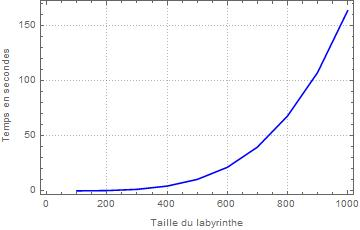
\includegraphics[width=\textwidth]{List_graph.jpg}
  \label{list}  
  \end{minipage}
  \hfill
  \begin{minipage}[h]{0.4\textwidth}
  \caption{Tree}
    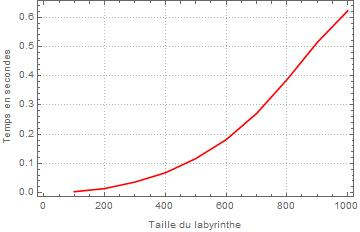
\includegraphics[width=\textwidth]{Tree_graph.jpg}
  \label{tree}
  \end{minipage}
  \begin{minipage}[h]{0.4\textwidth} 
  \caption{List et Tree}
    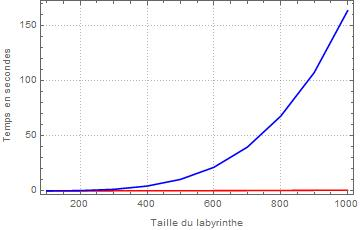
\includegraphics[width=\textwidth]{List_Tree_graph.jpg} 
  \label{listtree}   
  \end{minipage}
  \hfill
  \begin{minipage}[h]{0.4\textwidth}
  \caption{Tree grande taille}
    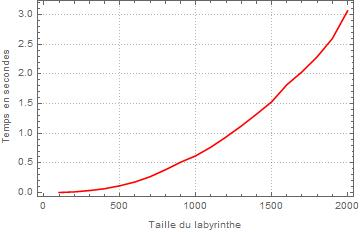
\includegraphics[width=\textwidth]{Tree_big_graph.jpg}
  \label{treebig}
  \end{minipage}
\end{figure}

%Dans la figure~\ref{étiquette}
\subsection{Analyse des résultats}
La figure \ref{list} montre que le temps de calcul croit très rapidement avec le carré de de la taille du labyrinthe. Ceci semble concorder avec les analyses théoriques combinées de l'\emph{unionFindList} et de \emph{mzCreate}.
\\

Sur la figure \ref{tree} on peut remarquer que l'implémentation de \emph{unionFindTree} croit très lentement, presque linéairement à partir de la taille 800. Des test plus nombreux furent réalisés ce qui donna la figure \ref{treebig}. On y voit que la courbe croit très lentement. Le temps dédié aux opération Union et Find devant être constant en pratique (démontré en 1989 par Fredman et Saks), on peut supposer que la légère croissance vient des opérations de \emph{mzCreate}.
\\

La comparaison entre l'implémentation \emph{List} et \emph{Tree} illustrée par la figure \ref{listtree} montre que la structure en arbre est bien plus performante. Pour un tableau de taille $1000$, $10^{6}$ éléments sont gérés par l'Union-Find. La génération du labyrinthe en utilisant la structure en liste nécessite 160 secondes, alors que celle en arbre ne prend que 0.6 secondes. Ceci est principalement dû aux améliorations implémentées à la structure en arbre (rang et compression de chemin).

\end{document}
